\documentclass[10pt,a4paper]{article}
\usepackage[margin=21mm,headheight=15pt]{geometry}
\usepackage[T1]{fontenc}
\usepackage{lmodern,amsmath,amssymb,tikz,graphicx,hyperref,fancyhdr,enumitem}
\usetikzlibrary{arrows.meta,positioning,calc,decorations.pathmorphing}
\definecolor{ink}{RGB}{20,53,78}
\hypersetup{colorlinks=true,urlcolor=ink,linkcolor=ink}
\setlength{\parindent}{0pt}\setlength{\parskip}{5pt}
\emergencystretch=3em
\pagestyle{fancy}\fancyhf{}\fancyfoot[C]{\thepage}
\renewcommand{\headrulewidth}{.3pt}
\newcommand{\task}[2]{\par\medskip{\color{ink}\Large\bfseries #1. #2}\par\smallskip}
\newcommand{\answer}{\par\smallskip\textbf{Worked reasoning.} }
\setlist[enumerate]{label=\textbf{(\alph*)},leftmargin=7mm,itemsep=7pt}
\begin{document}
\fancyhead[L]{\small Control of Dynamical Systems}
\fancyhead[R]{\small Laboratory 05}
{\color{ink}\LARGE\bfseries Laboratory 05}\par
{\large Flywheel speed regulation under a load torque}\par
\textbf{Exercise sheet -- five integrated problems}\par
{\small\textbf{Evidence boundary.} Original hypothetical scenarios. Derive, calculate and justify decisions; every numerical record is synthetic. Figures are conceptual and not to scale.}
\smallskip\textbf{Shared nominal data.} Motor: $R=2\,\Omega$, $L=0.02$ H, $J=0.01$ kg m$^2$, $b=0.02$ N m s/rad and $k_t=k_e=0.1$ in consistent SI units. The nominal load is 0.03 N m. Saturation applies only where explicitly stated.
\par\smallskip{\small\textbf{Study route.} Begin with balances, power and P/PI behavior. Problem 4(a,c) uses Routh stability from Laboratory 06; Problem 1(b) previews controllability developed in Laboratory 10. These are planned return tasks.}
\task{1}{From armature current to flywheel motion}
The illustrated DC motor drives a flywheel against bearing friction and an opposing load. Identify the two energy stores and distinguish back emf from mechanical load torque.
\begin{center}\resizebox{\ifdim\width>.98\linewidth.98\linewidth\else\width\fi}{!}{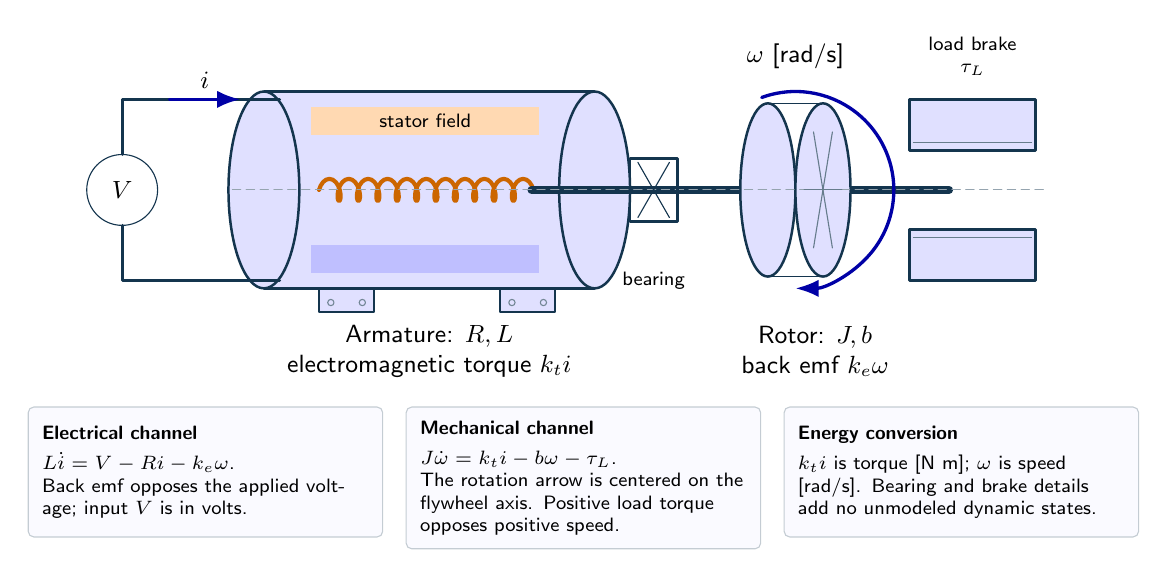
\begin{tikzpicture}[
font=\sffamily\small,>=Latex,line cap=round,line join=round,
wall/.style={draw=ink,line width=1.2pt,fill=blue!5},
water/.style={fill=cyan!25,draw=none},
metal/.style={draw=ink,fill=blue!12,line width=.9pt},
flow/.style={->,draw=blue!65!black,line width=1.2pt},
heat/.style={->,draw=orange!85!black,line width=1.1pt},
measure/.style={->,draw=teal!70!black,line width=.9pt},
dim/.style={<->,draw=ink!65,line width=.6pt},
spring/.style={draw=ink,decorate,decoration={coil,aspect=.5,segment length=4pt,amplitude=3pt}},
wire/.style={draw=ink,line width=1pt},
lab/.style={align=center,font=\sffamily\small},
smalllab/.style={align=center,font=\sffamily\scriptsize}]

\draw[metal](3,1.4)rectangle(7.2,3.9);
\draw[metal](3,2.65)ellipse(.45 and 1.25);
\draw[metal](7.2,2.65)ellipse(.45 and 1.25);
\fill[orange!30](3.6,3.35)rectangle(6.5,3.7);
\fill[blue!25](3.6,1.6)rectangle(6.5,1.95);
\node[smalllab]at(5.05,3.53){stator field};
\draw[orange!80!black,line width=1.5pt,decorate,decoration={coil,segment length=7pt,amplitude=4pt}](3.7,2.65)--(6.5,2.65);
\draw[ink,line width=3pt](6.4,2.65)--(11.7,2.65);
\draw[metal](9.4,2.65)ellipse(.35 and 1.1);
\draw[metal](10.1,2.65)ellipse(.35 and 1.1);
\draw[ink](9.4,3.75)--(10.1,3.75)(9.4,1.55)--(10.1,1.55);
\draw[metal](11.2,1.5)rectangle(12.8,2.15);
\draw[metal](11.2,3.15)rectangle(12.8,3.8);
\node[smalllab]at(12,4.35){load brake\\$\tau_L$};
\draw[flow]($(9.75,2.65)+(110:1.25)$)arc[start angle=110,end angle=-90,radius=1.25];
\node[lab]at(9.75,4.35){$\omega$ [rad/s]};
\draw[wire](3.2,3.8)--(1.2,3.8)--(1.2,3.1)(3.2,1.5)--(1.2,1.5)--(1.2,2.2);
\draw[ink](1.2,2.65)circle(.45);
\node at(1.2,2.65){$V$};
\draw[flow](1.8,3.8)--(2.7,3.8)node[midway,above]{$i$};
\node[lab]at(5.1,.6){Armature: $R,L$\\electromagnetic torque $k_t i$};
\node[lab]at(10,.6){Rotor: $J,b$\\back emf $k_e\omega$};
% REFINED EQUIPMENT DETAILS

% Motor feet, bearing blocks, shaft centerline and flywheel spokes.
\draw[metal](3.7,1.1)rectangle(4.4,1.4);\draw[metal](6,1.1)rectangle(6.7,1.4);
\foreach \x in {3.85,4.25,6.15,6.55}{\draw[ink!60](\x,1.22)circle(.04);}
\draw[ink!45,densely dashed](2.6,2.65)--(12.9,2.65);
\draw[metal,fill=none](7.65,2.25)rectangle(8.25,3.05);
\draw[ink](7.75,2.3)--(8.15,3)(7.75,3)--(8.15,2.3);
\foreach \a in {0,60,...,300}{\draw[ink!65](10.1,2.65)--++({.24*cos(\a)},{.85*sin(\a)});}
\draw[ink!65](11.25,3.25)--(12.75,3.25)(11.25,2.05)--(12.75,2.05);
\node[smalllab]at(7.95,1.5){bearing};

\node[draw=ink!25,fill=blue!2,rounded corners=2pt,anchor=north west,text width=4.15cm,minimum height=1.65cm,inner sep=5pt,align=left,font=\sffamily\scriptsize]at(0.0,-0.1){\textbf{Electrical channel}\\[3pt]$L\dot i=V-Ri-k_e\omega$.\\Back emf opposes the applied voltage; input $V$ is in volts.};
\node[draw=ink!25,fill=blue!2,rounded corners=2pt,anchor=north west,text width=4.15cm,minimum height=1.65cm,inner sep=5pt,align=left,font=\sffamily\scriptsize]at(4.8,-0.1){\textbf{Mechanical channel}\\[3pt]$J\dot\omega=k_ti-b\omega-\tau_L$.\\The rotation arrow is centered on the flywheel axis. Positive load torque opposes positive speed.};
\node[draw=ink!25,fill=blue!2,rounded corners=2pt,anchor=north west,text width=4.15cm,minimum height=1.65cm,inner sep=5pt,align=left,font=\sffamily\scriptsize]at(9.6,-0.1){\textbf{Energy conversion}\\[3pt]$k_ti$ is torque [N m]; $\omega$ is speed [rad/s]. Bearing and brake details add no unmodeled dynamic states.};
\end{tikzpicture}
}\par{\small A voltage-driven motor converts armature current into shaft torque. The rotor and external brake introduce inertia, friction and load torque. The illustrative cutaway does not add magnetic saturation or friction to the stated linear model.}\end{center}
\begin{enumerate}
\item A motor has $R=2\,\Omega$, $L=0.02$ H, $J=0.01$ kg m$^2$, $b=0.02$ N m s/rad and $k_t=k_e=0.1$ in SI units. Define voltage $v$, current $i$, speed $\omega$ and opposing load torque $d$. Derive the two balance equations and both speed transfer functions.
\item Use $x=[i,\omega]^T$ and voltage as control input. Write A, B and the load-input vector. Compute the determinant of the controllability matrix and interpret it.
\item Explain why controllability of the linear state model does not guarantee that a requested motion can be produced by a voltage-limited supply. Identify the missing constraint in an unconstrained controllability calculation.
\end{enumerate}
\vfill{\small\textbf{Submission.} Show the model, intermediate reasoning, units and a conclusion addressing the stated requirements.}

\newpage
\task{2}{Checking both torque and power at the supply limit}
Before tuning feedback, determine whether the requested speed and load are physically compatible with the supply. Use equilibrium and energy balance as independent checks.
\begin{enumerate}
\item Find the current and voltage required to hold 5 rad/s against 0.03 N m load. If available voltage is limited to 2 V, find the largest sustainable positive speed for that load.
\item At 5 rad/s and 0.03 N m load, calculate electrical input power, copper loss, viscous dissipation and useful load power. Verify conservation using the equilibrium from Problem 2(a).
\item At the largest loaded equilibrium speed permitted by a 2 V supply, calculate current, electrical input power, copper loss, viscous loss and useful load power. Verify their sum.
\end{enumerate}
\vfill{\small\textbf{Submission.} Show the model, intermediate reasoning, units and a conclusion addressing the stated requirements.}

\newpage
\task{3}{Proportional tracking versus integral load rejection}
Compare proportional and PI regulation of the same loaded flywheel. The controller's internal integral state is a voltage contribution, not an additional physical energy source.
\begin{center}\resizebox{\ifdim\width>.98\linewidth.98\linewidth\else\width\fi}{!}{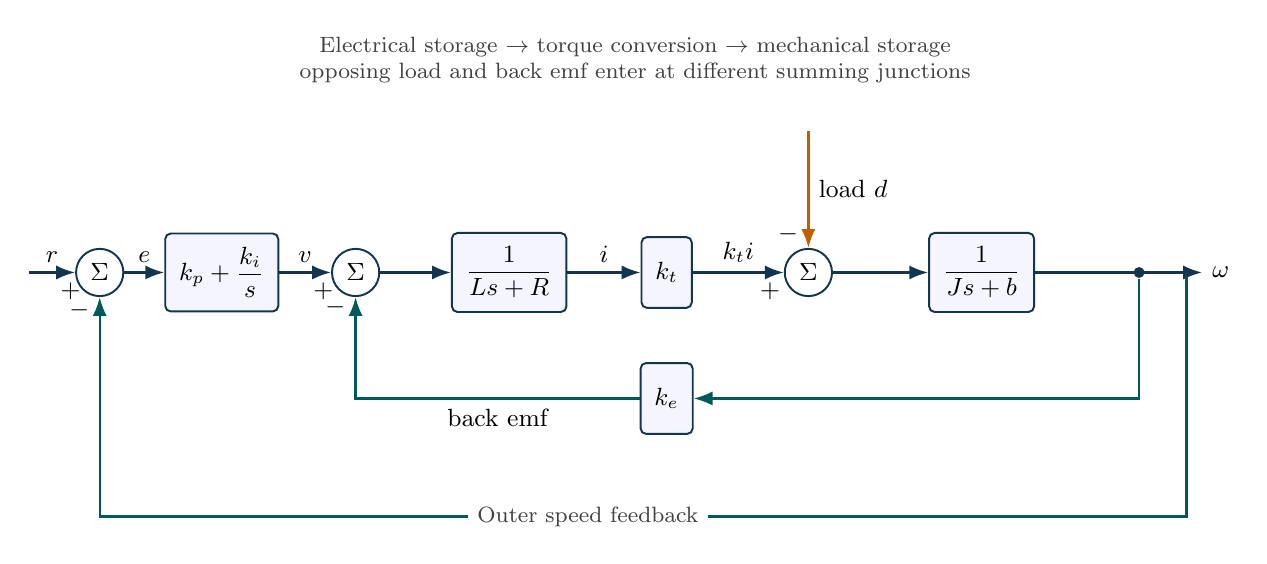
\begin{tikzpicture}[x=1cm,y=1cm,>=Latex,font=\small,
block/.style={draw=ink,fill=blue!4,rounded corners=2pt,minimum height=9mm,align=center,line width=.7pt,inner sep=5pt},
sum/.style={circle,draw=ink,fill=white,minimum size=6mm,inner sep=0pt,line width=.7pt},
sig/.style={->,draw=ink,line width=.85pt},
fb/.style={->,draw=teal!70!black,line width=.85pt},
dist/.style={->,draw=orange!75!black,line width=.85pt},
tap/.style={circle,fill=ink,inner sep=1.4pt},
note/.style={font=\footnotesize,align=center,text=black!75}]

\node[sum](e)at(.8,0){$\Sigma$};
\node[block](c)at(2.35,0){$k_p+\dfrac{k_i}{s}$};
\node[sum](v)at(4.05,0){$\Sigma$};
\node[block](el)at(6,0){$\dfrac{1}{Ls+R}$};
\node[block](kt)at(8,0){$k_t$};
\node[sum](tau)at(9.8,0){$\Sigma$};
\node[block](mech)at(12,0){$\dfrac{1}{Js+b}$};
\node[tap](w)at(14,0){};
\draw[sig](-.1,0)--node[above]{$r$}node[pos=.9,below]{$+$}(e);
\draw[sig](e)--node[above]{$e$}(c);
\draw[sig](c)--node[above]{$v$}node[pos=.85,below]{$+$}(v);
\draw[sig](v)--(el);
\draw[sig](el)--node[above]{$i$}(kt);
\draw[sig](kt)--node[above]{$k_ti$}node[pos=.85,below]{$+$}(tau);
\draw[sig](tau)--(mech);
\draw[sig](mech)--(14.8,0)node[right]{$\omega$};
\draw[dist](9.8,1.8)--node[right]{load $d$}node[pos=.88,left]{$-$}(tau);
\node[block](ke)at(8,-1.6){$k_e$};
\draw[fb](w)--(14,-1.6)--(ke);
\draw[fb](ke)--node[below]{back emf}(4.05,-1.6)--node[pos=.9,left]{$-$}(v);
\draw[fb](14.6,0)--(14.6,-3.1)--(.8,-3.1)--node[pos=.94,left]{$-$}(e);
\fill[ink](14.6,0)circle(1.4pt);
\node[note,fill=white]at(7,-3.1){Outer speed feedback};
\node[note]at(7.6,2.7){Electrical storage $\rightarrow$ torque conversion $\rightarrow$ mechanical storage\\opposing load and back emf enter at different summing junctions};

\end{tikzpicture}
}\par{\small Outer PI speed regulation around the electromechanical motor. The inner back-emf path and opposing load torque have explicit negative signs.}\end{center}
\begin{enumerate}
\item Use $v=k_p(r-\omega)$ with $k_p=0.8$, constant reference $r=5$ and load $d=0.03$. Find the equilibrium speed and tracking error from the physical equilibrium relation.
\item Replace the controller by $v=k_p(r-\omega)+z$, $\dot z=k_i(r-\omega)$, with $k_p=0.8$, $k_i=1.6$. Find the equilibrium speed and integral state for $r=5$, $d=0.03$. State the conditions needed to use this equilibrium as a final-value prediction.
\item Restore the 2 V supply constraint while retaining the 5 rad/s reference. What equilibrium claim from the ideal PI design becomes invalid, and what can anti-windup legitimately improve?
\end{enumerate}
\vfill{\small\textbf{Submission.} Show the model, intermediate reasoning, units and a conclusion addressing the stated requirements.}

\newpage
\task{4}{A stable PI controller has two different closed-loop channels}
Controller tuning changes reference tracking and load rejection through a shared denominator, but different numerators. Check stability before applying final-value arguments.
\begin{enumerate}
\item Derive the strict stability condition for positive PI gains. Decide whether $(k_p,k_i)=(0.8,1.6)$ and $(0.8,150)$ satisfy it, and interpret the equality boundary.
\item For an arbitrary stabilizing controller C, derive $\Omega/R$ and $\Omega/D_{load}$. Evaluate the latter at zero frequency for proportional gain 0.8 and for a stable PI controller with nonzero integral gain.
\item For $k_p=0.8$, impose the additional design rule that $k_i$ must stay at least 20 percent below its Routh upper boundary. Calculate the allowed positive interval and assess $k_i=1.6$. Explain what this rule does not measure.
\end{enumerate}
\vfill{\small\textbf{Submission.} Show the model, intermediate reasoning, units and a conclusion addressing the stated requirements.}

\newpage
\task{5}{A reduced model and a load estimate during acceleration}
The electrical time scale is short compared with the nominal mechanical one. Decide what may be neglected in a speed model and what must still be retained when estimating load.
\begin{enumerate}
\item Set L to zero and derive the reduced voltage-to-speed model and its time constant. Compare that time constant with $L/R$. Explain why this scale comparison is not a universal proof that inductance can be ignored.
\item Derive a steady load estimate using measured voltage and speed. Find the load-estimate error caused separately by a +0.1 V voltage bias and a +0.1 rad/s speed bias.
\item Starting from the full balances, derive the exact load torque in terms of measured voltage, speed and their state derivatives. Find the transient bias in the steady load estimator and explain why noise complicates correcting it.
\end{enumerate}
\vfill{\small\textbf{Submission.} Show the model, intermediate reasoning, units and a conclusion addressing the stated requirements.}

\end{document}
